\chapter{Future Linear Colliders}
\label{chapter:colliders}

\epigraph{Progress is not a straight line.}{An Wang}

In the post-LHC era, the major unanswered questions in particle physics centre around the Higgs boson and its properties, the identification of additional sources of CP-violation that can account for the universe's abundance of matter and paucity of antimatter, and the discovery of physics beyond the Standard Model. There are many investigations into each of these fields that utilise the Large Hadron Collider, or will leverage the upgrades for the \acrfull{HL-LHC}. However, now that the Higgs boson has been identified successfully, one of the most fruitful avenues for further research is the construction and operation of a lepton collider with sufficient centre-of-mass energy to produce Higgs bosons in larger numbers. [...]

These are the primary motivations for the construction of future colliders, especially lepton colliders, to succeed the Large Hadron Collider. The two main candidates are the \acrfull{ILC} and the \acrfull{CLIC}. Since both are linear eletron-positron colliders, they share many features, design considerations, and challenges, 

%Yn yr oes wedyn-LHC, y cwestiynau anatebedig mawr yn ffiseg gronnynau yn canolbwyntio o gwmpas y boson Higgs a'i nodweddion, y [identification] o unrhwy ffynonellau ychwanegol o CP-anghadwaith sy'n gallu esbonio'r gormodedd o sylwedd a'r anamledd o gwrth-sylwedd yn y cydfyd, a'r darganfod o ffiseg tros y Model Safonol. Mae llawer o [investigations] i mewn i pob un o'r [fields] yma sy'n defynddio'r Large Hadron Collider, neu bydd [leverage] y [upgrades] ar gyfer yr LHC gyda [luminosity] uchel (LHC-?U).

\section{Introduction}
[...]

\section{The physics case for a lepton collider}
[...]

Measurements of particles and their properties will be made significantly easier and thus more precise in the cleaner final state environment of a lepton collider, allowing for precision measurements of the Standard Model, putting better limits on the existence of new physics. It will also allow high-precision measurements of the properties of the Higgs boson, allowing linear colliders to determine their properties very precisely. Multiple BSM models rely upon properties of the Higgs being different from those predicted by the Standard Model, and 

%Bydd mesuron o ronynnau a'u nodweddion yn haws mawr a felly manolach yn yr ystad gorffenol glanach o wrthdarwr llinellol, gadael mesuruon manoldeb o'r Model Safonol, gwneud terfynau gwell ar gyfer y bodolaeth o ffiseg newydd. Bydd hefyd gadael uchel-manoldeb mesuron o'r nodweddion o'r boson Higgs, gadael gwrthdarwr llinellol i benderfynu eu nodweddion yn manwl iawn. Lluos o fodelau Tros y Model Safonol (TMS) yn sefyll y bod y nodweddion o'r Higgs yn gwahanol na'r rheiny wedi daroganu gan y Model Safonol.

\section{The International Linear Collider}

The \acrfull{ILC} is a proposed high-luminosity linear electron-positron collider, designed to have an initial energy of between 200-500 GeV, upgradable to 1 TeV at a later date. The ILC and its detectors are designed with the intention of becoming a "Higgs factory" -- producing large numbers of Higgs bosons to allow more detailed study of these particles.

There were a number of proposed sites for the ILC, including CERN in Geneva, DESY in Hamburg, and \acrshort{JINR} near Moscow. Due to the 2008 economic crisis, the United States and United Kingdom severely cut funding for linear collider projects, and this resulted in Japan stepping up to offer to host the collider in the Kitakami Highlands region of Iwate prefecture. This is partially due to a commitment the Japanese government made in [year] to cover half of the cost of construction, commissioning and operation if it was hosted within Japan.

However as of writing, a report from the Science Council of Japan (a representative organisation of the Japanese science community) released in 2019 expressed that they have not reached a consensus as to whether to support hosting the ILC in Japan. Some  of the reasons cited were concerns over international cost-sharing in the long-term, as well as to whether the expected scientific outcomes would justify the unprecedented human resource requirements and infrastructure necessary to make the ILC a reality \cite{linearcolliders-scj-report}.

The final decision to host the ILC will be made by the Japanese government's Ministry of Education, Culture, Sports, Science and Technology (MEXT), [...]

\subsection{The ILD and SiD detectors}
[...]

One of the unique features of the ILC is the push-pull detector system. This is a moving platform in the chamber housing the interaction point, upon which two detectors can be mounted. The platform can be moved to change which detector is in the beamline, allowing a linear collider to function with multiple detectors. Switching detectors is expected to take [some] hours. This allows the two detectors to specialise for different physics studies and goals, much like the experiments at the Large Hadron Collider at CERN, which is normally not possible with linear colliders. [?] [...]

\subsubsection{The International Large Detector (ILD)}
[...]

\begin{figure}[h]
	\centering
	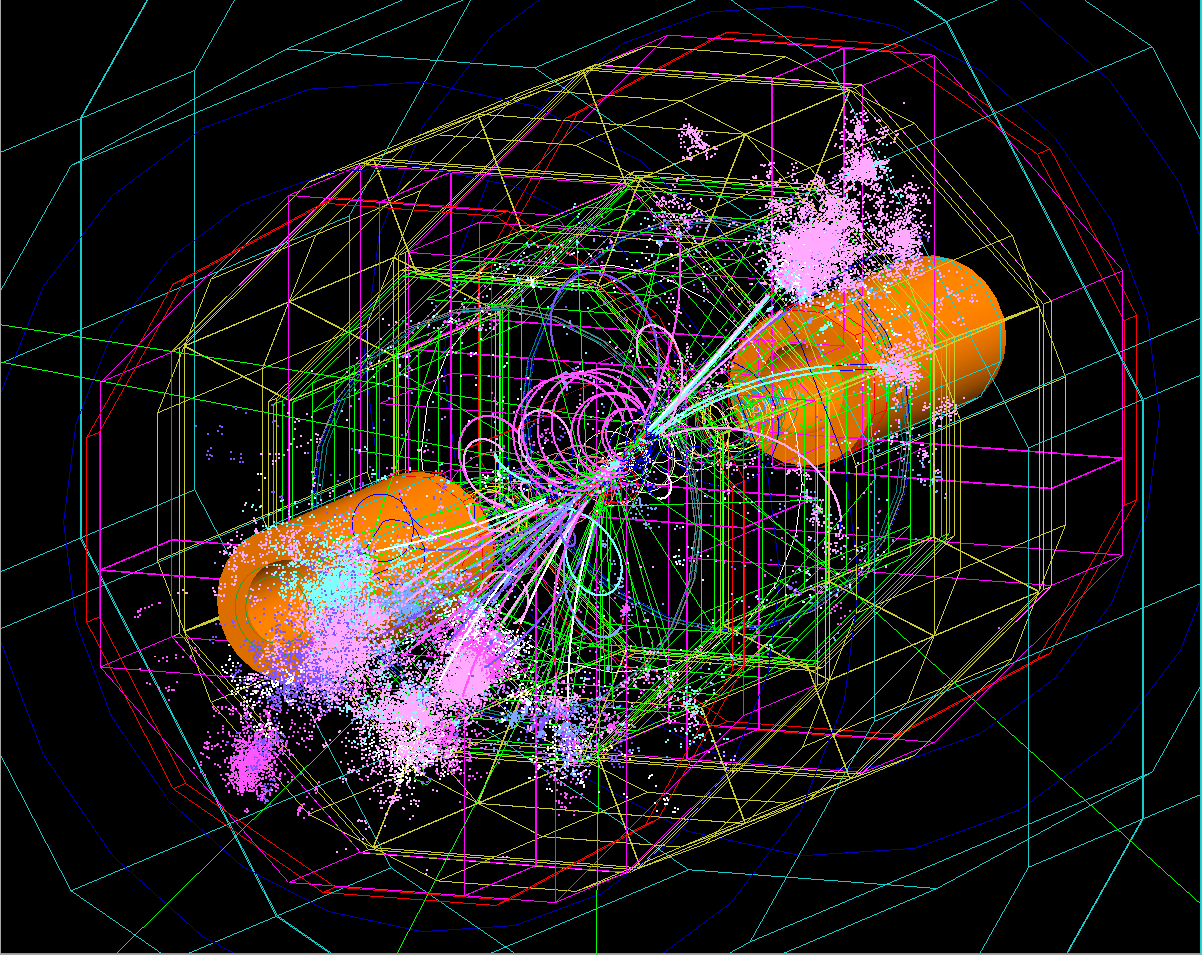
\includegraphics[width=0.75\textwidth]{../Pictures/SimulatedEvent1.png}
	\caption{Visualisation of a simulated tth event in the ILD. Charged particles can be easily identified by their curved, coiled or spiral paths, and the jets are clearly visible as the light pink and purple areas near the beampipes on either side.}
	\label{figure:colliders/ILD/tth-simulation}
\end{figure}

\subsubsection{The Silicon Detector (SiD)}
[...]

\section{The Compact Linear Collider}
[...]

[...] CLIC would be built beneath the existing LHC ring at CERN, stretching across the French-Swiss border and running parallel to the feet of the Jura mountain range. [...]

As of writing, the CLIC project has been submitted as input for the European Particle Physics Strategy Update, which will decide which projects the CERN collaboration chooses to pursue from 2020  onwards. [...]

CLIC's initial centre-of-mass energy will be 380 GeV, with successive upgrades increasing it to 1.5 TeV and 3 TeV. 